\documentclass[../../main.tex]{subfiles}
\usepackage[italian]{babel}

\begin{document}
    
\chapter{Introduzione}

Il cloud computing è un modello di distribuzione dei servizi informatici che consente di accedere a risorse e applicazioni tramite Internet, senza doverle mantenere localmente sul proprio computer o server. 
Attraverso il cloud computing, le risorse come l'archiviazione dei dati, la potenza di calcolo e il software vengono forniti come servizi virtuali da parte di fornitori specializzati, noti come provider di cloud(Amazon,Google ecc.).\\
La peculiarità sta nel fatto che le risorse vengono istanziate su richiesta, generalmente sotto forma di macchine virtuali.
I provider gestiscono l'infrastruttura fisica e mettono a disposizione degli utenti le risorse necessarie in base alle loro esigenze. In questo modo, le aziende possono evitare di investire in costosi hardware e software, riducendo i costi operativi e aumentando la flessibilità.

\section{Cloud Computing}
Possiamo distinguere diverse tipologie di servizi cloud in base al tipo di risorse che vengono fornite:
\subsection{Infrastructure as a Service}
L'Infrastructure as a Service (IaaS) è un modello di cloud computing che fornisce risorse informatiche virtualizzate tramite Internet. Con l'IaaS, i provider di cloud mettono a disposizione degli utenti l'infrastruttura fisica necessaria, inclusi server virtuali, storage, reti e altre risorse, consentendo loro di creare e gestire l'ambiente informatico in modo flessibile e scalabile.
Attraverso l'IaaS, gli utenti possono evitare di dover investire in hardware e infrastrutture costose, riducendo i costi di gestione e manutenzione. I provider di cloud si occupano dell'acquisizione, dell'installazione e della gestione dell'hardware, nonché della fornitura delle risorse virtuali agli utenti. Questo modello consente alle aziende di concentrarsi sullo sviluppo delle proprie applicazioni e servizi, piuttosto che preoccuparsi dell'infrastruttura sottostante.
La peculiarità sta nel fatto che le risorse vengono istanziate su richiesta o domanda di una piattaforma che ne ha bisogno.

\subsection{Platform as a Service}
Il Platform as a Service (PaaS) offre un ambiente di sviluppo e di esecuzione completo per le applicazioni. I provider di cloud mettono a disposizione degli sviluppatori un insieme di strumenti, framework e servizi che semplificano il processo di sviluppo, test e distribuzione delle applicazioni.
PaaS offre un'ampia gamma di strumenti di sviluppo, come linguaggi di programmazione, framework e ambienti di sviluppo integrati (IDE), che semplificano il processo di sviluppo delle applicazioni. Gli sviluppatori possono scrivere il codice, testare e distribuire le applicazioni direttamente nell'ambiente fornito dal PaaS, senza dover configurare manualmente l'infrastruttura.
Alcuni esempi di questo modelli li troviamo in Google App Engine, Microsoft Azure App Service e AWS Elastic Beanstalk.

\subsection{Software as a Service}
Il Software as a Service(SaaS) è modello di cloud computing che fornisce agli utenti applicazioni basate su cloud attraverso Internet. Con il SaaS, i provider di cloud ospitano e gestiscono l'infrastruttura e i software applicativi, consentendo agli utenti di accedere e utilizzare le applicazioni tramite Internet, senza dover installare il software sul proprio computer.
Consiste nell'utilizzo di programmi installati su un server remoto, cioè fuori del computer fisico o dalla LAN locale, spesso attraverso un server web; l'utente può accedere al programma tramite un browser web, come se fosse un programma installato localmente.
I modelli di pagamento del SaaS sono spesso basati sul consumo effettivo delle risorse, consentendo agli utenti di pagare solo per ciò che effettivamente utilizzano. Questo modello di pricing basato su abbonamento o utilizzo può essere vantaggioso per le aziende, in quanto consentono di evitare costi iniziali elevati e di prevedere meglio i costi operativi.
Alcuni esempi più comuni di SaaS li troviamo in Google Workspace, Microsoft Office 365, Dropbox.
\subsection{Function As a  Service}
Function as a Service(FaaS) è un modello di cloud computing che consente agli sviluppatori di eseguire e gestire le proprie funzioni senza dover gestire l'infrastruttura sottostante.
In FaaS, gli sviluppatori suddividono le loro applicazioni in funzioni modulari e indipendenti. Ogni funzione esegue un'attività specifica e può essere attivata in risposta a eventi o richieste specifiche. Ad esempio, una funzione può essere scatenata da un evento di caricamento di un file su un sistema di archiviazione cloud, da una richiesta HTTP o da un timer programmato. Quando una funzione viene attivata, il fornitore di servizi cloud gestisce automaticamente la sua esecuzione, inclusa la gestione delle risorse necessarie. Le funzioni vengono eseguite in ambienti isolati e scalati automaticamente in base alle richieste di carico. Una volta completata l'esecuzione della funzione, le risorse vengono deallocate per massimizzare l'efficienza e minimizzare i costi.
FaaS è diventato un'opzione popolare per lo sviluppo di microservizi, serverless application e scenari di elaborazione event-driven, fornendo un modo flessibile ed efficiente per eseguire singole funzioni di codice.
L'utente sostanzialmente deve solo fornire la logica aziendale insieme alle sue dipendenze e il fornitore del cloud è responsabile dell'allocazione di risorse, della scalabilità e della disponibilità del servizio. Queste piattaforme vengono generalmente fatturate in base al consumo, consentendo agli sviluppatori di ridurre i costi aumentando al tempo stesso l'agilità.\autocite{bhatt2022study}
Alcuni esempi di FaaS li troviamo in AWS Lambda, Google Cloud Functions, Azure Functions.

\subsubsection{Serverless Computing}
Serverless computing rappresenta un paradigma che va oltre il semplice Function-as-a-Service (FaaS), in cui il fornitore di servizi cloud si occupa completamente della gestione dell'infrastruttura sottostante. Il FaaS è un sottoinsieme del Serverless computing che si concentra specificamente sulla gestione delle singole funzioni come entità indipendenti. In questo contesto, le funzioni vengono eseguite in modo scalabile e senza che l'utente debba preoccuparsi della gestione diretta dell'infrastruttura sottostante.\autocite{amslaurea24930}\\
Nel serverless computing, il provider cloud si occuperà di allocare le risorse necessarie per eseguire il codice e di deallocarle una volta terminata l'esecuzione. Questo facilita la distribuzione e la scalabilità del sistema, cercando di automatizzare quest'ultima fase.
Focalizzandoci in questa gestione delle risorse, viene introdotto un linguaggio cAPP che ci permetterà di sincronizzare le risorse attraverso determinate politiche.\autocite{DBLP:journals/corr/abs-1902-03383}
\newpage
\section{Allocation Priority Policies}
Partiamo da un linguaggio dichiarativo APP(\textit{Allocation Priority Policies})\autocite{de2020allocation} che ci permette di definire politiche di allocazione delle risorse per le funzioni serverless, derivato da un estensione dello scheduler di OpenWhisk.
Vediamo qui di seguito un esempio del funzionamento:
\begin{figure}[H]
   \centering
    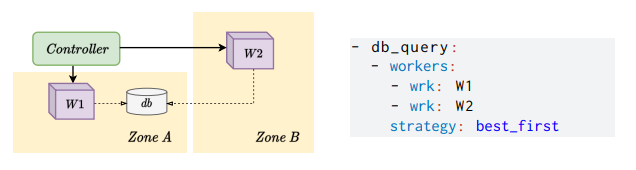
\includegraphics{ServerlessSchedulingPoliciesExample.png}
    \caption{Esempio di sistema serverless basato su APP}
\end{figure}
A destra troviamo il codice dichiarativo APP che fornisce le regole per allocare/invocare le funzioni: abbiamo due \textbf{Workers} che sono disponibili, e una strategia che regola come allocare queste risorse nei rispettivi worker; inoltre una \textbf{Strategy} che determina come allocare le risorse e secondo quale priorità.
Attualmente però la strategy ci permette di allocare secondo poche strategie generiche gia consolidate.
L'obiettivo diventa ora automatizzare questo processo, definendo le politiche di scheduling utilizzando le informazioni derivate dall'analisi statica delle funzioni che dovranno essere eseguite, per definire le politiche di allocazione delle risorse.
Osserviamo adesso un'altro esempio andando ancor di più in profondità:\\
Data una grammatica definita nel paper \autocite {deserverless}, osserviamo alcuni esempi di funzioni:
\begin{lstlisting}[language=Java, caption= La guardia della condizione è un espressione,label={lst:1}]
    (isPremiumUser, par) => {
        if (isPremiumUser) {
           call PremiumService(par)
        } else {
            call BasicService(par)
        }
    }
\end{lstlisting}

Il parametro \textit{isPremiumUser} è un valore che indica se l'utente richiede il servizio premium o meno, e in base a questo valore viene eseguita una chiamata o l'altra.
Di conseguenza assumiamo che il ramo condizionale prende il massimo della latenza tra le due chiamate, non sappiamo staticamente se verrà eseguito il ramo \textit{then} o \textit{else} e quindi non possiamo preventivare il tempo di esecuzione della funzione.

\begin{lstlisting}[language=Java, caption= La guardia della condizione è un'invocazione a un servizio esterno,label={lst:2}]
    (username, par) => {
        if (call isPremiumUser(username)) {
            call PremiumService(par)
        } else {
            call BasicService(par)
        }
    }
\end{lstlisting}

Nel caso sopra riportato invece, se l'utente che scatena l'evento è un membro premium, il tempo di esecuzione previsto dalla funzione è la somma delle latenze delle invocazioni dei servizi \textit{isPremiumUser} e \textit{PremiumService}.
Quindi possiamo preventivare il ritardo atteso(come tempo di esecuzione peggiore), cioè la somma della latenza del servizio \textit{isPremiumUser} più il massimo tra la latenza dei servizi \textit{PremiumService} e \textit{BasicService}.\\
Osserviamo ora un esempio di funzione con logica Map-Reduce:

\begin{lstlisting}[language=Java, caption=Funzione con logica Map-Reduce,label={lst:3}]
    (jobs, m, r)=>{
        for(i in range(0,m)){
            call Map(jobs, i)
            for(j in range(0,r)){
                call Reduce(jobs, i, j)
            }
        }
    }
\end{lstlisting}
Il parametro jobs descrive una sequenza di lavori map-reduce, dove il numero dei jobs è indicato dal parametro m.
La fase di \textit{Map} che genera m sottotask ``ridotti'' è implementata da un servizio esterno \textit{Map} che riceve jobs e un indice i che indica il job mappato.
Per ogni i, ci sono j sottotask.
In questo caso ci aspettiamo che la latenza dell'intera funzione è data dalla somma di m volte la latenza di \textit{Map} e m $\times $ r volte la latenza di \textit{Reduce}.\autocite{de2023custom}\\
\subsection{cAPP}
\label{cApp}
cAPP è un estensione di APP, dove le politiche di schedulazioni delle funzioni dipendono dai costi associati alle possibili esecuzioni delle funzioni sui worker disponibili\autocite {deserverless}.
cAPP è stato modificato al fine di implementare nuovi costrutti quali \textit{min\_latency} e \textit{max\_latency} che ci permettono di definire un upper bound e un lower bound per la latenza di una funzione.
\begin{multicols}{2}
    \begin{lstlisting}[caption={cAPP for Listing \ref{lst:1} e \ref{lst:2}},label={lst:4}]
-premUser:
    -workers:
        -wrk: W1
        -wrk: W2
    strategy: min_latency
    \end{lstlisting}
    \columnbreak
    \begin{lstlisting}[caption={cAPP for Listing~\ref{lst:3}}, label={lst:5}]
-mapReduce:
    -workers:
        -wrk: W1
        -wrk: W2
    strategy: random
    invalidate:
        strategy: max_latency
    \end{lstlisting}
\end{multicols}

Nel Listing \ref{lst:4}, osserviamo come diamo la possibilità di allocare la funzione \textit{premUser} su due workers, e la strategia di allocazione è quella di minimizzare la latenza, ovvero di dare priorità al worker su cui la soluzione dell'espressione di costo è minima.
Illustriamo però meglio le fasi della tecnica di \textit{min\_latency}:\\
Quando viene creato lo script cAPP, viene creata l'associazione tra il codice delle funzioni e il loro script etichettando le funzioni con \textit{//tag:premUser}.
Successivamente abbiamo bisogno del calcolo delle funzioni di costo, il codice delle funzioni viene utilizzato per dedurre i programmi di costo corrispondenti.
Quando le funzioni vengono invocate, possiamo calcolare la soluzione del programma di costo data la conoscenza dei parametri di invocazione.
Quando riceviamo una richiesta ad esempio per il Listing \ref{lst:1} prendiamo il suo programma di costo (rappresentato dal punto di intersezione sinistra) e la corrispondente politica cAPP per implementare la politica di schedulazione prevista.
Questa politica può essere ottenuta in due fasi: Calcolando i programmi di costo dal Solver, eseguendoli in ogni worker, e scegliendo il worker che ha latenza minima per contattare il \textit{PremiumService}.
Invece nel caso del Listing \ref{lst:5}, abbiamo una strategia di invalidazione \textit{max\_latency}, dopo aver selezionato un worker con una determinata strategia, andiamo a verificare se il worker è in grado di eseguire la funzione andando a risolvere l'espressione di costo corrispondente sostituendo i parametri $m$ e $r$ con la latenza dei servizi \textit{Map} e \textit{Reduce} dal worker selezionato e verifichiamo che la latenza sia inferiore a quella definita nello script.\autocite{deserverless}
\begin{figure}[H]
    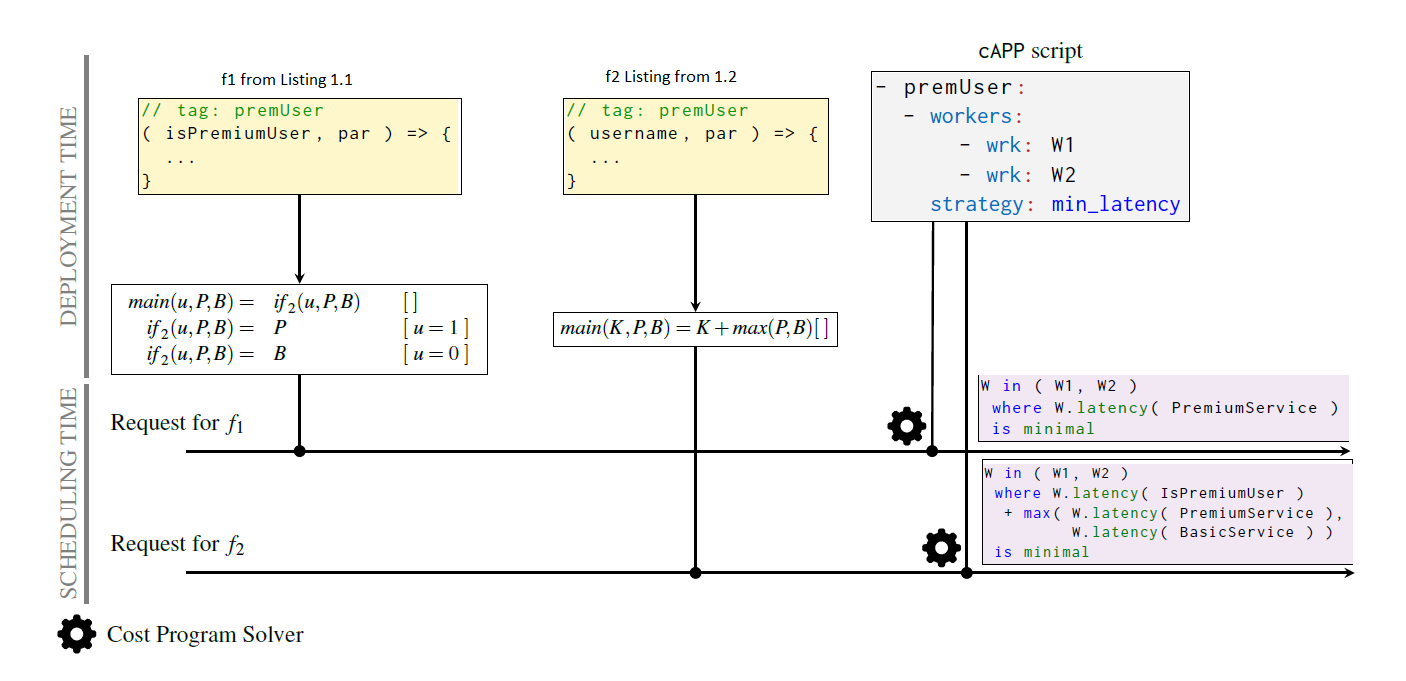
\includegraphics[width=.9\textwidth]{SchedulingDeployFlow.png}
    \centering
    \caption{From Deploy to Scheduling for Listing \ref{lst:1} e \ref{lst:2} }
\end{figure}

\section{Obiettivo della tesi}
L'obiettivo principale della tesi è approfondire le tecniche utilizzate per analizzare la semantica delle funzioni scritte in un linguaggio specifico, il quale sarà dettagliatamente delineato nei capitoli successivi. Tale analisi semantica è cruciale per generare le equazioni di costo associate a ciascuna funzione. Queste equazioni di costo forniscono dati fondamentali, come la complessità, che rappresenta un limite superiore delle prestazioni della funzione stessa. Queste informazioni sono essenziali per ottimizzare l'esecuzione delle funzioni serverless una volta richieste, consentendo un'allocazione efficiente delle risorse e una riduzione dei tempi di esecuzione.

Il percorso di ricerca si articola in diverse fasi. Innanzitutto, sarà definita una grammatica specifica per il linguaggio di programmazione in questione. Successivamente, verrà sviluppato un interprete per tale linguaggio, in grado di analizzare un programma scritto in un linguaggio ad alto livello e di restituire le relative equazioni di costo per ciascuna funzione. Inoltre, verrà generato il corrispondente codice WebAssembly, pronto per essere eseguito in un ambiente serverless.
WebAssembly svolge un ruolo cruciale come ambiente di esecuzione per il codice generato dalle nostre analisi di costo. Utilizzando il WebAssembly come target per le nostre ottimizzazioni, possiamo garantire una maggiore portabilità e interoperabilità delle nostre soluzioni, consentendo l'esecuzione efficiente delle funzioni serverless in una varietà di ambienti di runtime.
Una volta ottenute le equazioni di costo, ci concentreremo sull'analisi dettagliata di ciascuna funzione, impiegando strumenti specifici come PUBS (Pratical Upper Bounds Solver) e CoFloCo (Cost Flow Complexity Analysis). Tali strumenti, menzionati rispettivamente nella letteratura \autocite{albert2008automatic} e \autocite{flores2014resource}, sono progettati per calcolare il limite superiore delle prestazioni delle funzioni, date le rispettive equazioni di costo. Quest'analisi approfondita ci fornirà una comprensione più dettagliata delle prestazioni delle funzioni, permettendoci di ottimizzare ulteriormente l'allocazione delle risorse e il processo di scheduling delle esecuzioni.
\end{document}